\section{The Poke and Projective Collapse}
\label{sec:poke}

While routine dynamics sustain relational superposition, an explicit intervention
breaks the coherence of the state vector. This section formalizes the \emph{poke},
states the projective collapse rule, establishes renormalization after partner
exit, and proves structural irreversibility.

\subsection{Taxonomy of Pokes}
\label{subsec:poke-taxonomy}

Empirically, a poke $\poke$ enters the system through one of three channels:
\begin{enumerate}[nosep]
  \item \textbf{Direct verbal poke ($\poke_{\mathrm{dir}}$).} A partner issues an
        unambiguous status query (``so what are we?'', ``are we dating
        exclusively?'') that blocks evasive deflection.
  \item \textbf{Indirect structural poke ($\poke_{\mathrm{ind}}$).} An unavoidable
        calendar collision, public event invitation, or shared holiday requires
        $W$ to grant visible rank~$1$ status to one partner while excluding others.
  \item \textbf{Accidental third-party poke ($\poke_{\mathrm{acc}}$).} A mutual
        acquaintance, tagged photograph, or misdirected message exposes concurrent
        involvement to one or more partners simultaneously.
\end{enumerate}

\subsection{The Poke Rule and Three-Phase Collapse}
\label{subsec:poke-rule}

\begin{principle}[The Poke Rule]
\label{prin:poke-rule}
Given a pre-poke system state $\ket{\Psi} = \sum_{i=1}^n a_i \ket{G_i}$ with
$\sum_{i=1}^n \abs{a_i}^2 = 1$, a non-cascading direct poke $\poke$ projects the
system onto a single primary branch:
\begin{equation}
  \ket{\Psi} \;\xrightarrow{\;\poke\;}\; \ket{G_k},
  \qquad \text{with probability } \Prob(k \mid \Psi, \poke) = \abs{a_k}^2 = w_k.
  \label{eq:collapse}
\end{equation}
\end{principle}

The probability that partner $G_k$ survives as the collapsed primary choice is
governed by his pre-poke weight $\abs{a_k}^2$, not by his intensity in any
isolated secondary role such as $r_2$ or $r_3$. Consequently, a partner who
invests heavily in late-night emotional labor can still face a low collapse
probability if his overall system amplitude $a_k$ remains smaller than that of
the primary baseline partner.

In behavioral observation, collapse unfolds across three sequential phases
illustrated in \cref{fig:collapse}:
\begin{enumerate}[nosep]
  \item \textbf{Phase 1: Silence.} Immediately following $\poke$, message response
        latency spikes ($\tau_s$) while $W$ evaluates competing obligations and
        computes which branch to retain.
  \item \textbf{Phase 2: Projective selection and redistribution.} If the social
        graph is sparse ($q < q_c$), $W$ commits to a single outcome $\ket{G_k}$
        with probability $\abs{a_k}^2$ or removes the poking partner and
        renormalizes weights over the remaining pool.
  \item \textbf{Phase 3: Social cascade (decoherence).} If partners communicate
        across a sufficiently connected friend graph ($q \ge q_c$), the poke
        triggers cross-partner verification and all active amplitudes decay
        toward zero ($\ket{\Psi} \to \ket{\emptyset}$).
\end{enumerate}

\begin{figure}[htbp]
  \centering
  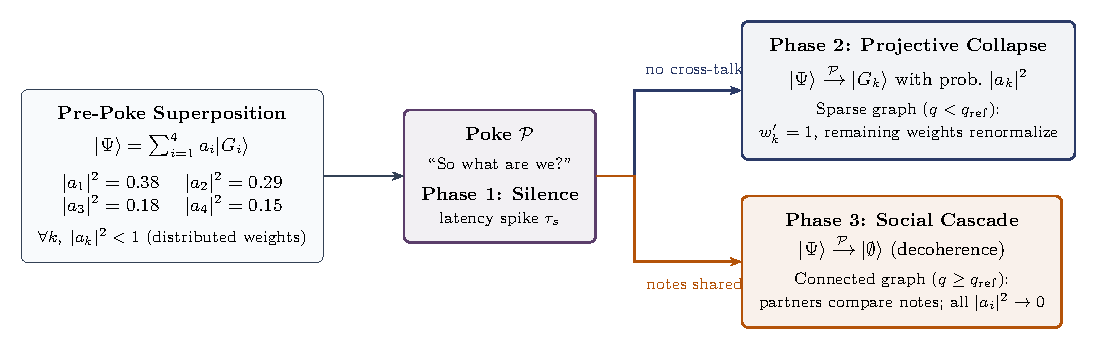
\includegraphics[width=0.95\textwidth]{figures/fig_collapse.pdf}
  \caption{State transition under a poke $\poke$. Left: pre-poke superposed state
  $\ket{\Psi}$ across four partners with primary weights $\abs{a_i}^2 < 1$.
  Center: silence latency during recomputation. Right: branching between isolated
  projective collapse $\ket{G_k}$ (top) and social-graph decoherence $\ket{\emptyset}$
  when partners compare notes (bottom).}
  \label{fig:collapse}
\end{figure}

\subsection{Post-Collapse Weight Redistribution}
\label{subsec:poke-redistribution}

When a poking partner $G_k$ rejects non-exclusivity and exits the portfolio
without triggering a system-wide cascade, $W$ redistributes attention across the
remaining partners $\partnerset \setminus \{G_k\}$.

\begin{proposition}[Validity of post-removal renormalization]
\label{prop:renormalization}
Let $\mathbf{w} = (w_1, \dots, w_n)$ satisfy $w_i \ge 0$ and $\sum_{i=1}^n w_i = 1$.
Suppose partner $G_k$ satisfies $w_k < 1$ (which holds automatically in any
superposed state by \cref{prop:nobody-first}). Define the post-removal weight
vector $\mathbf{w}'$ by
\begin{equation}
  w'_i = \begin{cases}
    0, & i = k, \\[4pt]
    \dfrac{w_i}{1 - w_k}, & i \neq k.
  \end{cases}
  \label{eq:renormalization}
\end{equation}
Then $w'_i \ge 0$ for all $i$, $w'_k = 0$, and $\sum_{i=1}^n w'_i = 1$. More
generally, for any retained subset $S \subseteq \{1, \dots, n\}$ with remaining
mass $M_S = \sum_{i \in S} w_i > 0$, setting $w''_i = w_i / M_S$ for $i \in S$
and $0$ otherwise preserves non-negativity and unit normalization.
\end{proposition}
\begin{proof}
Since $w_k < 1$, the denominator $1 - w_k > 0$ is strictly positive, so
$w'_i \ge 0$ for all $i$. Summing over $i \neq k$ gives
\begin{equation*}
  \sum_{i=1}^{n} w'_i
  = \sum_{i \neq k} \frac{w_i}{1 - w_k}
  = \frac{1}{1 - w_k} \sum_{i \neq k} w_i
  = \frac{1 - w_k}{1 - w_k} = 1.
\end{equation*}
The subset statement follows identically by dividing by $M_S > 0$.
(Machine-checked in Lean~4 as \texttt{RST.removePartner\_sum\_one} and
\texttt{RST.renormMask\_valid}.)
\end{proof}

Notice a subtle consequence of~\eqref{eq:renormalization}: removing one partner
mechanically amplifies the relative collapse weights of all remaining partners
by the factor $(1 - w_k)^{-1} > 1$, moving remaining partners closer to dominance
even if none of their absolute behaviors changed.

\begin{example}[Post-exit weight amplification in a three-partner triad]
\label{ex:renorm-triad}
Return to the triad of \cref{ex:triad} with pre-poke weights
$\mathbf{w} = (0.45, 0.35, 0.20)$ and rank ambiguity entropy
$H_{\mathrm{rank}}(\mathbf{w}) = 1.513$ bits. Suppose emotional-support partner
$G_2$ ($w_2 = 0.35$) issues a direct poke demanding exclusivity, refuses an
ambiguous reply, and exits without triggering a social-graph cascade. Applying
renormalization~\eqref{eq:renormalization} with amplification factor
$(1 - 0.35)^{-1} = \frac{20}{13} \approx 1.5385$ yields
\begin{equation*}
  \mathbf{w}' = \left(\frac{0.45}{0.65},\; 0,\; \frac{0.20}{0.65}\right)
  = \left(\frac{9}{13},\; 0,\; \frac{4}{13}\right)
  \approx (0.6923,\; 0.0000,\; 0.3077).
\end{equation*}
Post-exit rank entropy drops from $1.513$ bits to
$H_{\mathrm{rank}}(\mathbf{w}') = h_2(9/13) \approx 0.890$ bits, and $G_1$'s
prospective collapse share jumps by $+24.2$ percentage points solely from
$G_2$'s departure.
\end{example}

\subsection{Irreversibility of Collapse}
\label{subsec:poke-irreversibility}

Practitioners frequently attempt to undo a poke through apologies, framing
retractions (``forget I asked''), or temporary withdrawal. Within \RST{},
however, collapse is structurally irreversible.

\begin{proposition}[Irreversibility and strict entropy collapse]
\label{prop:irreversibility}
Let $\ket{\Psi}$ be a superposed state with rank ambiguity entropy
$H_{\mathrm{rank}}(\mathbf{w}) > 0$. Under a projective poke selecting branch
$\ket{G_k}$, the post-poke weight vector $\mathbf{w}_{\mathrm{post}} = \mathbf{e}_k$
satisfies:
\begin{enumerate}[nosep]
  \item $H_{\mathrm{rank}}(\mathbf{w}_{\mathrm{post}}) = 0 < H_{\mathrm{rank}}(\mathbf{w})$;
  \item the transition $\mathbf{w} \mapsto \mathbf{e}_k$ is a many-to-one
        projection that erases all relative phase information $\{a_i / a_j\}$
        and pre-poke weight ratios among non-selected partners;
  \item even if $W$ subsequently re-adds new partners, the historical state
        $\ket{\Psi}$ cannot be reconstructed uniquely from $\ket{G_k}$ alone.
\end{enumerate}
\end{proposition}
\begin{proof}
In superposition, at least two weights satisfy $0 < w_i < 1$, so
$-w_i \log_2 w_i > 0$ and $H_{\mathrm{rank}}(\mathbf{w}) > 0$. After collapse to
$\ket{G_k}$, $w_{\mathrm{post}, k} = 1$ and $w_{\mathrm{post}, j} = 0$ for
$j \neq k$, giving $H_{\mathrm{rank}}(\mathbf{w}_{\mathrm{post}}) = -1 \log_2 1 = 0$.
Moreover, infinitely many distinct normalized vectors $\ket{\Psi}$ with
$a_k \neq 0$ project onto the same ray $\ket{G_k}$, so the collapse map has no
left inverse on the space of superposed states.
\end{proof}

Behaviorally, once a direct status answer has been forced into the shared
record between $W$ and $G_k$, the pre-poke ambiguity that permitted simultaneous
interpretations is no longer sustainable without overt contradiction.

\subsection{Sequential Rank-Role Queries and Order Dependence}
\label{subsec:poke-sequential}

In \cref{sec:uncertainty}, non-commutation $\comm{\opR}{\opL} \neq 0$ implied
that the order in which rank and role are asked changes the resulting state.
We now demonstrate this effect explicitly using projective measurements on a
two-partner system.

Suppose $\ket{\Psi} = \frac{3}{5}\ket{G_1} + \frac{4}{5}\ket{G_2}$ in the
rank basis $\{\ket{G_1}, \ket{G_2}\}$, and consider two orthogonal observables:
rank $\opR = \diag(1, 2)$ with eigenbasis $\{\ket{G_1}, \ket{G_2}\}$, and a
role-alignment observable $\opL_{\mathrm{align}}$ with orthonormal eigenstates
$\ket{\ell_+} = \frac{1}{\sqrt{2}}(\ket{G_1} + i\ket{G_2})$ and
$\ket{\ell_-} = \frac{1}{\sqrt{2}}(\ket{G_1} - i\ket{G_2})$.
\begin{enumerate}[nosep]
  \item \textbf{Protocol RL (ask rank first, then role).} Querying rank first
        collapses $\ket{\Psi}$ onto $\ket{G_1}$ with probability $\frac{9}{25} = 0.36$
        or $\ket{G_2}$ with probability $\frac{16}{25} = 0.64$. Conditional on
        either outcome, a subsequent role query yields $\ket{\ell_+}$ or $\ket{\ell_-}$
        with probability $\frac{1}{2}$ each, leaving the post-role state with
        equal weights $(\frac{1}{2}, \frac{1}{2})$ on $G_1$ and $G_2$ if rank
        is queried again.
  \item \textbf{Protocol LR (ask role first, then rank).} Querying role first
        yields $\abs{\braket{\ell_+}{\Psi}}^2 = \frac{1}{2}\abs{\frac{3}{5} - \frac{4}{5}i}^2 = \frac{1}{2}$
        and $\abs{\braket{\ell_-}{\Psi}}^2 = \frac{1}{2}$. In either post-role
        eigenstate $\ket{\ell_\pm}$, a subsequent rank query yields $G_1$ with
        probability $\frac{1}{2} = 0.50$ and $G_2$ with probability $\frac{1}{2} = 0.50$,
        completely erasing the initial $(0.36, 0.64)$ asymmetry!
\end{enumerate}
Protocol RL initially resolves $(0.36, 0.64)$ on rank before role inquiry
scrambles rank to $(0.50, 0.50)$, whereas Protocol LR yields $(0.50, 0.50)$ on
rank from the outset. Thus, probing a partner's functional role before asking
about priority genuinely alters the resulting rank distribution.

\subsection{Post-Collapse Survival and Re-Entry Conditions}
\label{subsec:poke-reentry}

If a system collapses onto $\ket{G_k}$ via \cref{prin:poke-rule}, can it ever
re-enter relational superposition when a new viable prospect $G_{n+1}$ arrives?
Technically, appending $G_{n+1}$ with small amplitude $\epsilon > 0$ produces
$\ket{\Psi'} = \sqrt{1 - \epsilon^2}\ket{G_k} + \epsilon\ket{G_{n+1}}$, which
mathematically satisfies \cref{def:superposition} if $\epsilon > 0$. However,
its rank ambiguity entropy is bounded by the binary entropy $h_2(\epsilon^2)$,
which remains negligible ($< 0.08$ bits for $\epsilon^2 \le 0.01$) unless
attention-drift dynamics (\cref{sec:dynamics}) drive $\epsilon^2$ above a
functional salience threshold $\tau_{\mathrm{sal}}$. By \cref{prop:irreversibility},
even if a fresh superposition forms around a new partner, the pre-poke coherent
state among the original partners cannot be restored.

